\documentclass{bioinfo}
\copyrightyear{2016}
\pubyear{2016}


\usepackage{pgf}
\usepackage{tikz}
\usepackage{adjustbox}
\usetikzlibrary{arrows,automata}

\usepackage{epsfig}
\usepackage{graphicx}
\usepackage{amsthm}
\usepackage{amssymb}
\usepackage{amsmath}
\usepackage{amsfonts}
\usepackage{mathrsfs,url}

\newcommand{\Oh}[1]
	{\ensuremath{\mathcal{O}\!\left({#1}\right)}}
\newcommand{\access}
	{\ensuremath{\mathsf{access}}}
\newcommand{\rank}
	{\ensuremath{\mathsf{rank}}}
\newcommand{\select}
	{\ensuremath{\mathsf{select}}}
\newcommand{\occ}
	{\ensuremath{\mathsf{occ}}}
\newcommand{\nodelabel}
	{\ensuremath{\mathsf{label}}}
\newcommand{\BWT}
	{\ensuremath{\mathsf{BWT}}}
\newcommand{\C}
	{\ensuremath{\mathsf{C}}}
\newcommand{\LF}
	{\ensuremath{\mathsf{LF}}}
\newcommand{\Psiop}
	{\ensuremath{\mathsf{\Psi}}}
\newcommand{\mus}[1]
	{\SI{#1}{\micro\second}}
	
\newcommand{\elabel}{\ensuremath{\mathsf{label}}}
\newcommand{\EBWT}{\ensuremath{\mathsf{EBWT}}}


\def\ours{\mbox{\rm {\sc Vari}}}


\begin{document}
\firstpage{1}

\title[Succinct Colored de Bruijn Graphs]{Succinct Colored de Bruijn Graphs}
\author[Muggli, Bowe \textit{et~al}]{
Martin D. Muggli\,$^{1,*}$, 
Alexander Bowe\,$^{2,*}$, 
Travis Gagie\,$^{3}$,
Robert Raymond\,$^{1}$,
Noelle R. Noyes\,$^{4}$,
Paul Morley\,$^{4}$,
Keith Belk\,$^{5}$,
Simon J. Puglisi\,$^{3}$, and Christina Boucher\,$^1$}
\address{$^{*}$These authors contributed equally to this work. \\
$^{1}$Department of Computer Science,Colorado State University, Fort Collins, CO \\
$^{2}$National Institute of Informatics, Chiyoda-ku, Tokyo, Japan \\
$^{3}$Department of Computer Science,University of Helsinki, Finland \\
$^{4}$Department of Clinical Sciences, Colorado State University, Fort Collins, CO \\
$^{5}$Department of Animal Sciences, Colorado State University, Fort Collins, CO }

\history{Received on XXXXX; revised on XXXXX; accepted on XXXXX}

\editor{Associate Editor: XXXXXXX}

\maketitle

\begin{abstract}
\section{Motivation:} Iqbal et al. (Nature Genetics, 2012) introduced the {\em colored de Bruijn graph}, a variant of the classic de Bruijn graph, which is aimed at ``detecting and genotyping simple and complex genetic variants in an individual or population''.
Because they are intended to be applied to massive population level data, it is essential that the graphs be represented efficiently.
Unfortunately, current succinct de Bruijn graph representations are not directly applicable to the colored de Bruijn graph, which require additional information to be succinctly encoded as well as support for non-standard traversal operations. 
\section{Results:} Our data structure dramatically reduces the amount of memory required to store and use the colored de Bruijn graph, with some penalty to runtime, allowing it to be applied in much larger and more ambitious sequence projects than was previously possible.  In particular, we use our method along with a custom curated database of antimicrobial resistant genes to track changes in the resistome across food production facilities. A short video of our work is available at \url{http://cdbg.martindmuggli.com}.

\end{abstract}


\section{Introduction}\label{sec:introduction}

In the 20 years since it was introduced to bioinformatics by Idury and Waterman~\cite{IW95}, the {\em de Bruijn graph} has become a mainstay of modern genomics, essential to genome assembly~\cite{how,sequel,ismb2015}. The near ubiquity of de Bruijn graphs has led to a number of succinct representations, which aim to implement the graph in small space, while still supporting fast navigation operations.  Formally, a de Bruijn graph constructed for a set of strings (e.g., sequence reads) has a distinct vertex $v$ for every unique $(k - 1)$-mer (substring of length $k - 1$) present in the strings, and a directed edge $(u, v)$ for every observed $k$-mer in the strings with $(k - 1)$-mer prefix $u$ and $(k - 1)$-mer suffix $v$. A contig corresponds to a non-branching path through this graph. See Compeau et al.~\cite{how} for a more thorough explanation of de Bruijn graphs and their use in assembly. 

In 2012, Iqbal et al.~\cite{ICTFM12} introduced the {\em colored de Bruijn graph}, a variant of the classical structure, which is aimed at ``detecting and genotyping simple and complex genetic variants in an individual or population.'' The edge structure of the colored de Bruijn graph is the same as the classic structure, but now to each vertex ($(k - 1)$-mer) and edge ($k$-mer) is associated a list of colors corresponding to the samples in which the vertex or edge label exists. More specifically, given a set of $n$ samples, there exists a set $\mathcal{C}$ of $n$ colors $c_1, c_2, .., c_n$ where $c_i$ corresponds to sample $i$ and all $k$-mers and $(k-1)$-mers that are contained in sample $i$ are colored with $c_i$. A {\em bubble} in this graph corresponds to a directed cycle, and is shown to be indicative of biological variation by Iqbal et al.~\cite{ICTFM12}. 
{\sc Cortex}, Iqbal et al.'s~\cite{ICTFM12} implementation, uses the colored de Bruijn graph to develop a method of assembling multiple genomes simultaneously, without losing track of the individuals from which $(k - 1)$-mers (and $k$-mers) originated as well as their coverage. This assembly is derived from either multiple reference genomes, multiple samples, or a combination of both.

Variant information of an individual or population can be deduced from structure present in the colored de Bruijn graph and the colors of each $k$-mer.
As implied by Iqbal et al.~\cite{ICTFM12}, the ultimate intended use of colored de Bruijn graphs is to apply it to massive, population-level sequence data that is now abundant due to next generation sequencing technology (NGS) and multiplexing. These technologies have enabled production of sequence data for large populations, which has led to ambitious sequencing initiatives that aim to study genetic variation for agriculturally and bio-medically important species.  These initiatives include the {\em Genome 10K} project that aims to sequence the genomes of 10,000 vertebrate species~\cite{Haussler:2009}, the {\em iK5} project~\cite{Robinson:2011}, the 150 Tomato Genome ReSequencing project~\cite{tomato1,tomato2}, and the 1001 Arabidopsis project, a worldwide initiative to sequence cultivars of {\em Arabidopsis}~\cite{arabidopsis}.   Given the large number of individuals and sequence data involved in these projects, it is imperative that the colored de Bruijn graph can be stored and traversed in a space- and time-efficient manner.


%\paragraph{Our Contributions and Results}  
We develop an efficient data structure for storage and use of the colored de Bruijn graph. Compared to {\sc Cortex}, Iqbal et al.'s~\cite{ICTFM12} implementation, our new data structure dramatically reduces the amount of memory required to store and use the colored de Bruijn graph, with some penalty to runtime. In addition to demonstrating the memory and runtime of $\ours$, we validate its output using the {\em E.coli} reference genomes and AMR dataset.  In particular, our experiment on the AMR dataset validates $\ours$'s ability to correctly identify AMR genes from a metagenomics sample, which  is of paramount importance since---when expressed in bacteria---AMR genes render the bacteria resistant to antibiotics and pose serious risk to public health.  Our experiments and results focus on beta-lactamases, which are genes that confer resistance to a class of antibiotics that are considered to be the last resort for infections from multi-drug-resistant bacteria \cite{mckenna,carbapenem_review}.  Our experiments demonstrate that all  beta-lactamases were correctly identified and only two of the remaining 47 genes were identified to be in the sample, which had 97\% and 95\% sequence similarity to one of the beta-lactamases in the sample.

\section{Related Work} As noted above, maintenance and navigation of the de Bruijn graph is a space and time bottleneck in genome assembly. Space-efficient representations of de Bruijn graphs have thus been heavily researched in recent years. One of the first approaches was introduced by Simpson et al.~\cite{Simpson:2009} as part of the development of the ABySS assembler.  Their method stores the graph as a distributed hash table and thus requires 336 GB to store the graph corresponding to a set of reads from a human genome (HapMap: NA18507). 
 
 In 2011, Conway and Bromage~\cite{conway} reduced space requirements  by using a sparse succinct bitvector (by Okanohara and Sadakane~\cite{bitvector}) to represent the $k$-mers (the edges), and used the characteristic \emph{rank()} and \emph{select()} operations to traverse it. As a result, their representation took 32 GB for the same data set.  Minia, by Chikhi and Rizk~\cite{wabi}, uses a Bloom filter to store edges. They traverse the graph by generating all possible outgoing edges at each node and testing their membership in the Bloom filter. Using this approach, the graph was reduced to 5.7 GB on the same dataset.  Contemporaneously, Bowe, Onodera, Sadakane and Shibuya~\cite{BOSS12} developed a different succinct data structure based on the Burrows-Wheeler transform~\cite{BW94} that requires 2.5 GB.  The data structure of Bowe et al.~\cite{BOSS12} is combined with ideas from IDBA-UD~\cite{idbaud} in a metagenomics assembler called MEGAHIT~\cite{megahit}.  In practice MEGAHIT requires more memory than competing methods  but produces significantly better assemblies.   Chikhi {et al.}~\cite{paul} implemented the de Bruijn graph using an FM-index and {\em minimizers}.   Their method uses 1.5 GB on the same NA18507 data.  In 2015, Holley et. al.~\cite{BFT} released the Bloom Filter Trie, which is another succinct data structure for the colored de Bruiin graph; however, we were unable to compare our method against it since  it only supports the building and loading of a colored de Bruijn graph and does not contain operations to support our experiments.  Lastly, SplitMEM~\cite{splitmem} is a related algorithm to create a colored de Bruijn graph from a set of suffix trees representing the other genomes. 


\section{Results}
We demonstrate this reduction in memory through a comprehensive set of bubble calling experiments across the following three datasets: (1) 3,765 {\em Escherichia coli (E. coli)} genome assemblies downloaded from NCBI, (2) a set of 54 antimicrobial resistance (AMR) genes and a simulated metagenomics sample containing seven of these 54 AMR genes, and four AMR genes not contained in this set, and, (3) four plant genomes.  We show our method, which we refer to as $\ours$ (Finnish for color), has better peak memory usage during graph traversal on all these datasets.  This observation is highlighted on two datasets: the plant reference genomes, where {\sc Cortex} required 101 GB and $\ours$ required 19 GB, and the set of \emph{E. coli} assemblies, which we could not successfully run {\sc Cortex} on (est. 3 TB for vertex storage) while $\ours$ completed traversal in 11 hours using only 26 GB. $\ours$ is a novel generalization of the succinct data structure for classical de Bruijn graphs due to Bowe et al.~\cite{BOSS12}, which is based on the Burrows-Wheeler transform of the sequence reads, and thus, has independent theoretical importance.

% \footnote{The supplement for \cite{ICTFM12} indicates 8b (k-mer) + 4b/color (coverage) + 1b (outgoing edges) for each of the 155M 31-mers.}
 
%the {\em Genome 10K} project that aims to sequence the genomes of 10,000 vertebrate species \cite{Haussler:2009}, the {\em iK5} project where the objective is to sequence the genomes of 5,000 arthropods \cite{Robinson:2011}, the 150 Tomato Genome ReSequencing project that aims to identify the sequence diversity within tomato \cite{tomato}, and the 1001 Arabidopsis  Project that is a worldwide initiative to sequence cultivars of Arabidopsis \cite{arabidopsis}. Given the large number of individuals and sequence data involved in these projects it is imperative that the colored de Bruijn graph is able to be stored and traversed in both a memory and time efficient manner.


 
 


%\section*{Preliminaries} \label{prel:vari}

As previously mentioned, in 2017 Muggli et al.~\cite{vari} presented $\vari$, which is a representation of the colored de Bruijn graph using BWT.  Our proposed method, $\ours$, efficiently merges de Bruijn graphs that are represented in this manner. Therefore, we first define some basic notation and definitions concerning BWT, then we show how the de Bruijn graph can be stored using BWT, and finally, we show how the {\em colored} de Bruijn graph can be stored succinctly.  We refer the reader to the full paper by Muggli et al.~\cite{vari} for a more detailed discussion of the representation.   

\subsection*{Basic Definitions and Terminology} %\subsection{sec:basic}

Here, we begin with some basic definitions related to our representation.  Throughout we consider a string $\X = \X[1..n] = \X[1]\X[2]\ldots
\X[n]$ of $|\X| = n$ symbols drawn from the alphabet $[0..\sigma-1]$.
%We assume $\X[n]$ is a special ``end of string'' symbol, \$, smaller than
%all other symbols in the alphabet.
For $i=1,\ldots,n$ we
write $\X[i..n]$ to denote the {\em suffix} of $\X$ of length $n-i+1$,
that is $\X[i..n] = \X[i]\X[i+1]\ldots \X[n]$.  
%We will often refer to suffix $\X[i..n]$ simply as ``suffix $i$''. 
Similarly, we write
$\X[1..i]$ to denote the {\em prefix} of $\X$ of length $i$.
$\X[i..j]$ is the {\em substring} $\X[i]\X[i+1]\ldots \X[j]$ of $\X$
that starts at position $i$ and ends at $j$. 
%By $\X[i..j)$ we
%denote $\X[i..j-1]$.  If $j < i$ we
%define $\X[i..j]$ to be the empty string, also denoted by
%$\varepsilon$.

\paragraph*{Suffix arrays and suffix array intervals.}
The suffix array~\cite{mm1993} $\SA_{\X}$ (we drop subscripts when
they are clear
from the context) of a string $\X$
is an array $\SA[1..n]$ which
contains a permutation of the integers $[1..n]$ such that $\X[\SA[1]..n]
\prec \X[\SA[2]..n] \prec \cdots \prec \X[\SA[n]..n]$.  In other words, $\SA[j] =
i$ if and only if $\X[i..n]$ is the $j^{\mbox{{\scriptsize th}}}$ suffix of $\X$
in lexicographical order. Here, $\prec$ denotes lexicographic precedence.

%The inverse
%suffix array $\ISA$ is the inverse permutation of $\SA$, that is
%$\ISA[i] = j$ iff $\SA[j] = i$.
%Conceptually, $\ISA[i]$ tells us the position of suffix $i$ in $\SA$. 

%Our data structure for colored de Bruijn graphs is based on a succinct representation of individual de Bruijn graphs that was introduced by Bowe et al.~\cite{BOSS12} and which we refer to as the BOSS representation from the authors' initials.  The BOSS representation was in turn based on an adaptation of Ferragina and Manzini's~\cite{FM05} FM-indexes.  Before getting to our description of the succinct colored de Bruijn graph data structure, 
%In the rest of this section 
%we first describe FM-indexes and then explain the BOSS representation.Our explanation of BOSS is particularly simple and may be of independent interest to those wanting to better understand that data structure.
% This new take on BOSS was key to our development of our succinct colored de Bruijn graph. 
% Travis: No it wasn't, it came afterward. :o)

For a string $\Y$, the $\Y$-interval in the suffix array $\SA_{\X}$ is
the interval $\SA[s..e]$ that contains all suffixes having $\Y$ as a
prefix. The $\Y$-interval is a representation of the occurrences of
$\Y$ in $\X$. For a character $c$ and a string $\Y$, the computation
of $c\Y$-interval from $\Y$-interval is called a \emph{left extension}.
%and the computation of $\Y$-interval from ${\Y}c$-interval is called a
%\emph{right contraction}. \emph{Left contraction} and \emph{right
%  extension} are defined symmetrically.

\paragraph*{BWT.} Next, for a string $\Y$, let $\F$ be the list of $\Y$'s characters sorted lexicographically by the suffixes starting at those characters, and $\L$ be the list of $\Y$'s characters sorted lexicographically by the suffixes starting immediately after those characters.  (The names $\F$ and $\L$ are standard for these lists.)  If \(\Y [i]\) is in position $p$ in $\F$ then \(\Y [i - 1]\) is in position $p$ in $\L$.  Moreover, if \(\Y [i] = \Y [j]\) then \(\Y [i]\) and \(\Y [j]\) have the same relative order in both lists; otherwise, their relative order in $\F$ is the same as their lexicographic order.  This means that if \(\Y [i]\) is in position $p$ in $\L$ then (assuming arrays are indexed from 0) in $\F$ it is in position
\[|\{h\,:\,\Y [h] \prec \Y[i]\}| + |\{h\,:\, \L [h] = \Y [i],\ h \leq p\}| - 1\,.\] Finally, notice that the last character in $\Y$ always appears first in $\L$.  It follows that we can recover $\Y$ from $\L$, which is the famous {\em Burrows-Wheeler Transform (BWT)}~\cite{bw1994} of $\Y$.


\paragraph*{FM-index and backward seach.}  Ferragina and Manzini~\cite{fm2005} first  realized BWT can be used for indexing in addition to compression.   Hence, if we know the range \(\BWT (\Y) [i..j]\) occupied by characters immediately preceding occurrences of a pattern $P$ in $\Y$, then we can compute the range \(\BWT (\Y) [i'..j']\) occupied by characters immediately preceding occurrences of \(c P\) in $\Y$, for any character $c$, since
\begin{eqnarray*}
i' & = & |\{h\,:\,\Y [h] \prec c\}| + |\{h\,:\,\Y [h] = c, h < i\}| \\
j' & =  & |\{h\,:\,\Y [h] \prec c\}| + |\{h\,:\, \Y [h] = c, h \leq j\}| - 1\,.
\end{eqnarray*}
Notice \(j' - i' + 1\) is the number of occurrences of \(c P\) in $S$.  The essential components of an FM-index for $\Y$ are: (1) an array storing \(|\{h\,:\,\Y [h] \prec c\}|\) for each character $c$ and, (2) a {\em rank} data structure for \(\BWT (\Y)\) that quickly tells us how often any given character occurs up to any given position. To be able to locate the occurrences of patterns in $\Y$ (in addition to just counting them), we can use a sampled suffix array of $\Y$ and a bitvector indicating the positions in \(\BWT (\Y)\) of the characters preceding the sampled suffixes.  

Hence, we define the function
$\rank(\Y, c,i)$, for string $\Y$, symbol $c$, and integer $i$, as 
the number of occurrences of $c$ in $\Y[1..i]$. Rank is used in {\em backward search}~\cite{fm2005} in order to compute left extension of a given string, i.e., the previous character. 

 %  It is well known that $\LF[i] = \C[\BWT[i]] + \rank(\BWT,\BWT[i],i)$.  Furthermore, we can compute the left extension using $\C$ and $\rank$.  If $\SA[s..e]$ is the $\Y$-interval,
%containing all the suffixes prefixed with string $\Y$,  then $\SA[\C[c]+\rank(\BWT,c,s),\C[c]+\rank(\BWT,c,e)]$ is the $c\Y$-interval. This is called \emph{backward search}~\cite{fm2005}, and a data structure supporting it is called an {\em FM-index}.


\subsection*{Storage of de Bruijn Graph using BWT} 

Given a de Bruijn graph $G =(V, E)$, we refer to the label of an edge $e \in E$ as the $k$-mer corresponding to it, and denote it as $\elabel(e)$.  Further, given $V$, we define the co-lexicographic (colex) ordering of $V$ as the lexicographic order of their reversed labels ($(k - 1)$-mers).  

We let $\F$ be the edges in $E$ in colex order by their ending nodes, where ties are broken by their starting nodes, and let $\L$ be the edges in $E$ sorted colex by their starting nodes, with ties broken by their ending nodes.  We refer to the ordering of $\L$ as {\em Vari-sorted}. If we are given two edges $e$ and $e'$ that have the same label then we are guaranteed that they have the same relative order in both $\F$ and $\L$; otherwise, their relative order in $\F$ is the same as their labels' lexicographic order.  This means that if $e$ is in position $p$ in $\L$, then in $\F$ it is in position
\[|\{d\,:\,d \in E,\ \elabel (d) \prec \elabel (e)\}| + \]
	\[ |\{h\,:\,\elabel (\L [h]) = \elabel (e),\ h \leq p\}| - 1\,\]
where $\prec$ denotes lexicographic precedence.  We define the edge-$\BWT$ ($\EBWT$) of $G$ to be the sequence of edge labels sorted according to the ordering of the edges in $\L$, so \(\elabel (\L [h]) = \EBWT (G) [h]\) for all $h$. Therefore, if we have an array $D$ storing \(|\{d\,:\,d \in E,\ \elabel (d) \prec c\}|\) for each character $c$ and  a fast rank data structure on \(\EBWT (G)\) then given an edge's position in $\L$, we can quickly compute its position in $\F$.

We let $\B_F$ be the bit vector with a 1 marking the position in $\F$ of the last incoming edge of each node, and let $\B_L$ be the bit vector with a 1 marking the position in $\L$ of the last outgoing edge of each node.  Given a character $c$ and the colex rank of a node $v$, we can use $\B_L$ to find the interval in $\L$ containing $v$'s outgoing edges.  We can then search \(\EBWT (G)\) to find the position of each outgoing edge\footnote{In practice, we incorporate the bits of $B_F$ as flags on \(\EBWT (G)\) and use them to obtain the colex order of $v$ but omit the discussion here for simplicity.  We refer the reader to Bowe et al.~\cite{BOSS} for a full discussion of this aspect and the supplement for our handling here.}. Similarly, we can make similar queries about the incoming edges of a node $v$ in an efficient manner using $\B_F$.  

%In addition, if $B_G$ is  the bit vector with a 0 marking the position in $\F$ of the first incoming edge of each node, we define $\flags$ to be the vector that stores the permutation from $\F$ to $\L$ applied to $\B_G$.  Next, we see how we use $\flags$.  If we are given a character $c$ and the colex rank of a node $v$, we can use $\B_L$ to find the interval in $\L$ containing $v$'s outgoing edges, then we can search in \(\EBWT (G)\) to find the position of the one $e$ labeled $c$.  We need $\flags$ in order to obtain the colex rank of $v$.  Thus, we can find $e$'s position in $\F$, as described above.  Finally, we can use $\B_F$ to find the co-lexicographic rank of $e$'s ending node.  

Therefore, briefly we explained how we can construct and represent a de Bruijn graph $G = (V, E)$ with $\EBWT$, $\B_L$,  and $\B_F$ in a manner that allows for efficient navigation of the graph. An example of this representation is shown in Figure \ref{fig:purple}. Given this representation we can traverse the graph and recover incoming and outgoing edges.   Next, we demonstrate how the labels ($k$-mers) can be recovered using this data structure.

%With the appropriate implementations of the data structures, we obtain the following result:
%\begin{theorem}[Bowe, Onodera, Sadakane and Shibuya, 2012]
%We can store $G$ in \((1 + o (1)) |E| (\lg \sigma + 2)\) bits such that, given a character $c$ and the co-%lexicographic rank of a node $v$, in $O{\log \log \sigma}$ time we can find the node reached from $v$ by following the directed edge labelled $c$, if such an edge exists.
%\end{theorem}

\paragraph*{Label recovery.}  We note that an important aspect of this succinct representation of the graph is that the $(k - 1)$-mers (nodes) and $k$-mers (edges) of the de Bruijn graph $G$ are not explicitly stored in the above representation---rather they than can be {\em computed} (or recovered) from this representation.    As previously mentioned, we can traverse the graph in a forward or reverse manner and recover incoming and outgoing edges of a given node $v$.  Given this efficient traversal, we can recover the label of $v$ by traversing the graph in a backward direction starting from $v$;  given the label of $v$ is a $(k - 1)$-mer we traverse backward $k - 1$ times.  Therefore, we must add extra nodes and edges to the graph to ensure there is a directed path of length at least \(k - 1\) to each original node.  More formally, we augment the graph so that each new node's label is a \((k - 1)\)-mer that is prefixed by one or more copies of a special symbol $\$$ not in the alphabet and lexicographically strictly less than all others.  When new nodes are added, we are assured that the node labeled $\$^{k - 1}$ is always first in colex order and has no incoming edges.  Lastly, we augment the graph in a similar manner by adding an extra outgoing edge, labeled $\$$, to each node with no outgoing edge.   These ``dummy nodes'' are shown in Figure \ref{fig:purple}.


%Here, we briefly describe the procedure for recovering these node and edge labels.  This method could be used for a trivial merge algorithm that we will discuss later.  

%If we know the range \(\B_L [i..j]\) of $k$-mers whose starting nodes end with a pattern $P$ of length less than \((k - 1)\), then we can compute the range \(\B_F [i'..j']\) of $k$-mers whose ending nodes end with \(P c\), for any character $c$, since
%\begin{eqnarray*}
%i' & = & |\{d\,:\,d \in E,\ \elabel (d) \prec c\}|  \\
 %  & & + |\{h\,:\,\EBWT (G) [h] = c,\ h < i\}|\\
%j' & = & |\{d\,:\,d \in E,\ \elabel (d) \prec c\}| \\
% &  & + |\{h\,:\,\EBWT (G) [h] = c,\ h \leq j\}| - 1\,.
%\end{eqnarray*}

%^Thus,  we can find the interval in $\B_L$ containing $v$'s outgoing edges in $O(k \log \log \sigma)$-time, provided there is a directed path to $v$ of length at least \(k - 1\) but note that we cannot use \(\EBWT (G)\), $\B_F$ and $\B_L$ alone to recover the labels of nodes with no incoming edges.  Thus, we add extra nodes and edges to the graph to ensure there is a directed path of length at least \(k - 1\) to each original node.  More formally, we augment the graph so that each new node's label is a \((k - 1)\)-mer that is prefixed by one or more copies of a special symbol $\$$ not in the alphabet and lexicographically strictly less than all others.  When new nodes are added, we are assured that the node labeled $\$^{k - 1}$ is always first in colex order and has no incoming edges.  Lastly, we augment the graph in a similar manner by adding an extra outgoing edge, labeled $\$$, to each node with no outgoing edge.  

\subsection*{Storage of Colors} 

Given a multiset \(\mathcal{G} = \{G_1, \ldots, G_t\}\) of individual de Bruijn graphs, we set $G$ to be the union of those individual graphs and build the previously described representation for $G$.  We also build and store a two-dimensional binary array $\C$ in which \(\C [i, j]\) indicates whether the $i$th edge in $G$ is present in the $j$th individual de Bruijn graph (i.e., whether that edge has the $j$th color).    Hence, we store a given de Bruijn graph using $\EBWT$, the described bit vectors, and a compressed color matrix.  The combination of the above storage of the graph $G$ plus the compressed matrix is the succinct storage of the graph. 



\begin{figure}
\centering
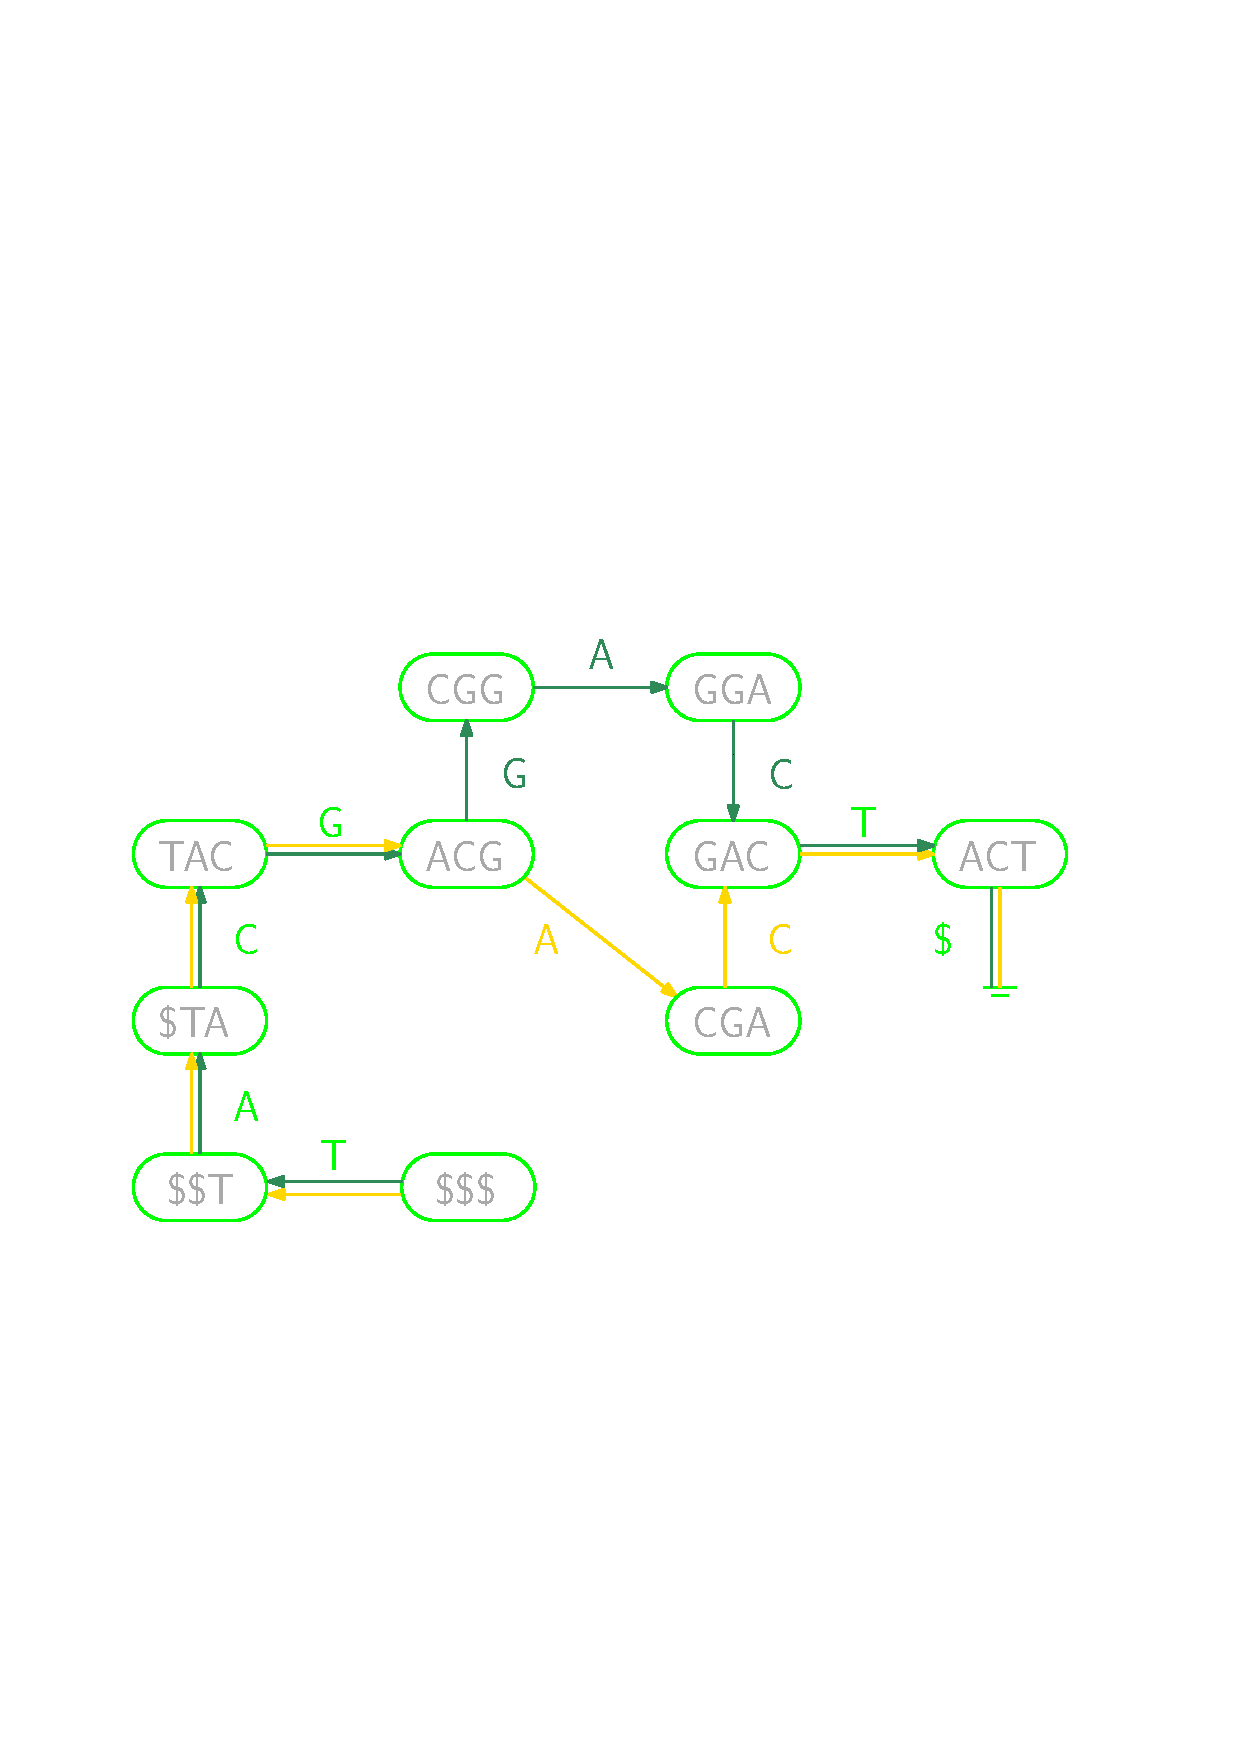
\includegraphics[width=.35\textwidth]{limegraph.pdf} \\~\\
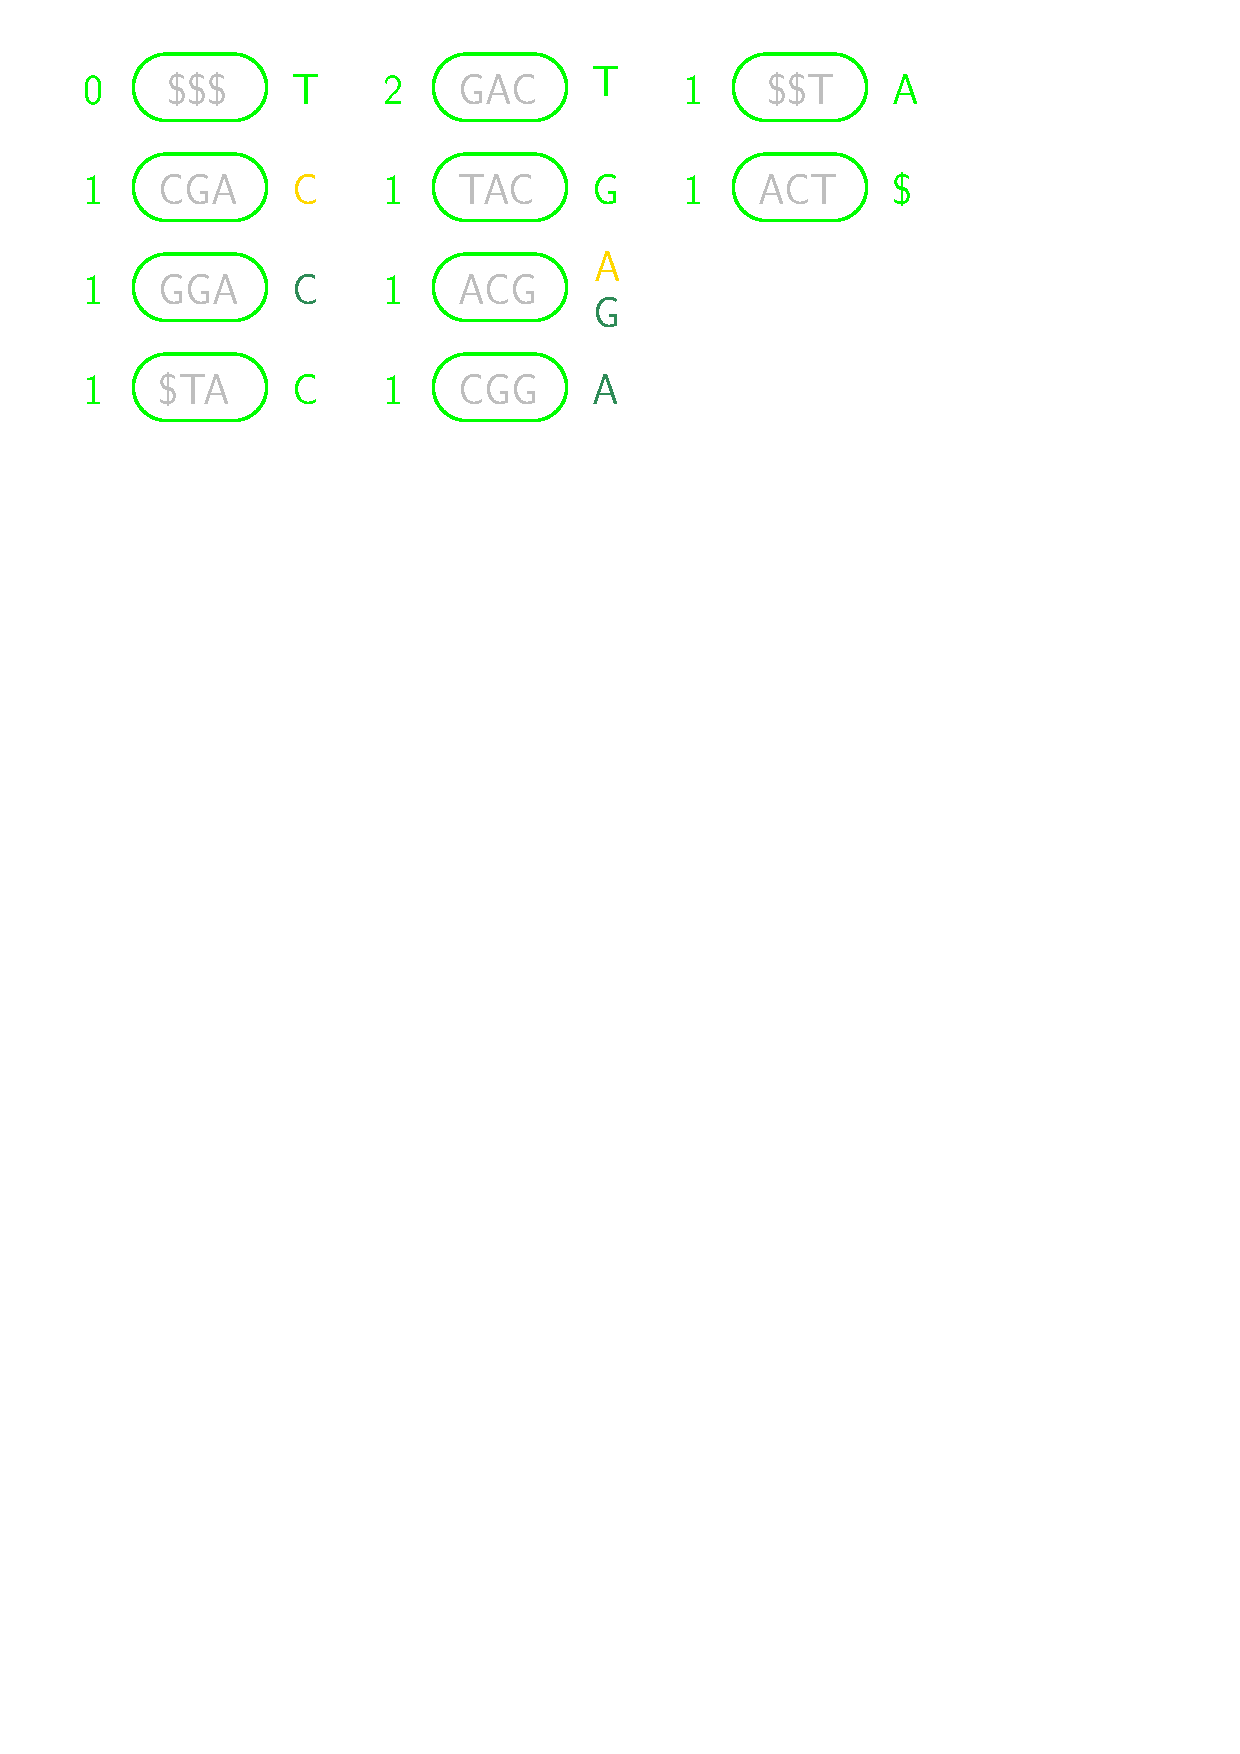
\includegraphics[width=.35\textwidth]{limeonlymapping.pdf} \\~\\
\raisebox{0.1ex}{$\begin{array}{rr}
   \EBWT (G) = &  \mathtt{TCCCTGAGAA\$}\\[1ex]
         \B_F = & \mathtt{ 1110111111}\\
         \B_L = & \mathtt{11111101111}\\[1ex]
C^\mathrm{T} = &   \mathtt{11011110011}\\
               &  \mathtt{10111101111}
\end{array}$}
%\end{tabular}
\caption{{\bf Top:} A colored de Bruijn graph consisting of two individual graphs, whose edges are shown in yellow and green. All nodes to be present in both graphs are shown in lime.  {\bf Below:} The $\vari$ representation of the colored de Bruijn graph: the edge-BWT and bitvectors for the union of the individual graphs, and the binary array $C$ (shown transposed) whose bits indicate which edges are present in which individual graphs.}
\label{fig:purple}
\end{figure}


%\begin{methods}
%\section{Methods}
%
%%%%%%%%%%%%%%%%%%%%%%%%%%%%%%%%%%%%%%%%
\section{Methods}\label{sec-meods}

We now describe the algorithm behind $\dopp$.
%, and some important implementation details.  
Three main insights enable our index-based aligner for Rmap data: 1) abstraction of the alignment problem to a finite automaton; 2) use of the GCSA for storing and querying the automaton; and 3) modification of backward search to use a wavelet tree in specific ways to account for the Rmap error profile.  %Casting the alignment problem as path matching in a finite automaton allows the first two errors (missing and false cut sites, and missing fragments) to be modelled.  The GCSA is an index-based data structure for storing and querying finite automaton.  The third type of error (inaccuracy in the fragment sizes) is taken into account by the use of the wavelet tree in the backward search algorithm. For simplicity we first describe standard backward search and then show how it can be extended. 

\subsection{Finite Automaton.}

Continuing with the example in the background section, we want to align $\R' = 6,5,3,5$ to $\R''' = 2,4,7,3,5$ and vice versa.  To accomplish this we cast the Rmap alignment problem to that of matching paths in a finite automaton.  A finite automaton is  a directed, labeled graph that defines a \emph{language}, or a specific set of sequences composed of vertex labels.  A sequence is recognized by an automaton if it contains a matching path: a consecutive sequence of vertex labels equal to the sequence. We represent the target Rmaps as an automaton and the query as a path in this context.  
%SJP: I didn't find this intuition at all helpful
%The intuition is as follows: we can construct an automaton where vertices represent compound fragments (groups of fragments), and the language comprises all the legal assignments of fragments to groups.  That is, every fragment of an Rmap is assigned to exactly one group. 

%\paragraph{Backbone}
The automaton for our target Rmaps can be constructed as follows.  First concatenate the $\R_1 \ldots \R_n$ together into a single sequence with each Rmap separated by  a special symbol which will not match any query symbol. Let $\R^*$ denote this concatenated sequence. Hence, $\R^* = [f_{11},..,f_{1m_1}, \ldots, f_{n1},..,f_{nm_n}]$.  Then, construct an initial finite automaton $\A = (V, E)$ for $\R^*$ by creating a set of vertices $v^i_1 .. v^i_m$, one vertex labeled with each fragment length and edges connecting them.% for each Rmap $\R_i$.
Also, introduce to $\A$  a {\em starting vertex} $v_1$ labeled with $\#$ and a {\em final vertex} $v_f$ labeled with the character $\$$.  All other vertices in $\A$ are labeled with integral values.  This initial set of vertices and edges is called the {\em backbone}.  The backbone by itself is only sufficient for finding alignments with no missing cut sites in the query. Figure \ref{fig:example}(a) illustrates the construction of $\A$ for a single Rmap.  The backbone of this automaton is $\#, 2, 3, 4, 5, 6, \$$.  Next, extra vertices (``skip vertices'') and extra edges are added to $\A$ to allow for the automaton to accept all valid queries.  

\paragraph{Skip Vertices and Skip Edges.}
We introduce additional vertices labeled with {\em compound fragments} to allow missing cut sites (first type of error) to be taken into account in querying the target Rmaps.  We refer to these as {\em skip vertices} as they provide alternative path segments which skip past two or more backbone vertices. Thus, we add a {\em skip vertex} to $\A$ for every $o+1$ length run of consecutive vertices in the backbone where $1 < o < order$ and  \emph{order} is the maximum number of consecutive missed cut sites to be accommodated.  First order skip vertices are each labeled with the sum of two consecutive backbone vertices.  Second order skip vertices are each labeled with the sum of three consecutive backbone vertices. The vertex labeled with $7$ connecting $2$ and $5$ in \ref{fig:example}(a) is an example of a skip vertex.  Likewise, $5, 9, 11$ are other skip vertices.

%The final state of a $\A$, then must additionally have a vertex for each proper compound fragment, such that all combinations are compactly encoded as paths from $v_1$ to $v_s$ in $\A$.


%\paragraph{Edges}
%In this automaton model, vertices represent compound fragments and edges represent restriction sites. Every restriction site in original target Rmaps is potentially conserved in aligning Rmap but the preceding and following sites may not be.  Thus, there will be multiple edges in our automaton corresponding to that site for every site in the original Rmap data: those joining two backbone vertices (edge $4 \rightarrow 5$), those joining skip vertices to backbone vertices (edges $5 \rightarrow 4$ and $3 \rightarrow 9$), and those joining skip vertices to each other (edge $5 \rightarrow 9$).  All matching paths that include one of the aforementioned edges conserve the cut site delimiting fragments $3$ and $4$ in the original Rmap.  
%For every site there will be a complete bipartite subgraph such that to match all possible missing site errors, an automaton will have $O(\ell \delta^2)$ edges, where $\ell$ is the concatenation of all Rmaps in the target and $\delta$ is the order.

Finally, we add {\em skip edges} which provide paths around vertices with small labels in the backbone.
%The dashed edges in figure \ref{fig:example} are the skip edges, which
These allow a query with a missing fragment to still match.\footnote{Different smallness thresholds for query and target bias toward this scenario, avoiding backtracking in the search.}  Hence, the addition of skip edges allow for desorption (the second type of error) to be taken into account in querying the target Rmaps.  


%This graph construction allows for any combination of missing and spurious restriction sites as well desorbed fragments.  As we explain below, when the automaton is indexed appropriately, inaccuracies in the fragment sizes (third type of error) can be handled efficiently, too. % I added the reason mid paragraph that occured at the end, maybe revert this change? -mm It reads well. - sjp
% are handled by using a {\em wavelet tree}.  The wavelet tree and the space succinct data structure used to implement the finite automaton for the  detection of alignments will be discussed in the next section.

\subsection{The Rmap Alignment Score.}

Alignments are found by incrementally extending candidate partial alignments (paths in the automaton) to longer partial alignments by choosing one of several compatible extension matches (adjacent vertices to the end of a path in the automaton).  To perform this search efficiently, we prune the search by a scoring model that scores the size agreement of the matched compound fragments, and the frequency of putative missing cut sites.

\paragraph{Size Agreement.}
We use the Chi-square CDF statistic to assess size agreement.  This assumes the fragment size errors are independent, normally distributed events.  For each pair of matched compound fragments in a partial alignment, we take the average between the two as the assumed true length and
% of the DNA that was measured.  Then we 
compute the expected standard deviation using this mean.  Each compound fragment deviates from the assumed true value by half the distance between them.  These two deviation values contribute two degrees of freedom to the Chi-square calculation.
%FIXME: include this as a formula

\paragraph{Cut Site Error Frequency.}
We use the Binomial CDF statistic to assess the probability of the number of cut site errors in a partial alignment.   This assumes missing cut site errors are independent, Bernoulli processes events.  We account for all the putatively conserved cut sites on the boundaries and those delimiting compound fragments in both partially aligned Rmaps plus twice the number of missed sites as Bernoulli trials. % Since our method handles both missing and false cuts, and false cuts are less frequent with common enzymes, we assume this scoring method is a sufficient approximation of the underlying process to work for our search.
%FIXME: include this as a formula

Thus, given a set of Rmaps and input parameters $\rho_{L}$ and $\rho_{U}$, we produce the set of all Rmap alignments that have a chi-square CDF statistic less than $\rho_U$ and a binomial CDF statistic less than $\rho_L$.  Both of these are subject to the additional constraint of a maximum consecutive missed restriction site run between aligned sites of $\delta$ and a minimum aligned site set cardinality of 16. 


%%As a result of allowing inexact matches, there may be multiple fragments in an optical map that could each be a reasonable match for an {\em in silico} digested fragment, and in order to include all of these as candidate matches, backtracking becomes necessary in the backward search.
%For every backward search path that maintains a non-empty interval for the entire query contig, we emit the alignments denoted by the final interval.%, mapped back to a position in the optical map.

\begin{figure*}[h!]
 \centering
 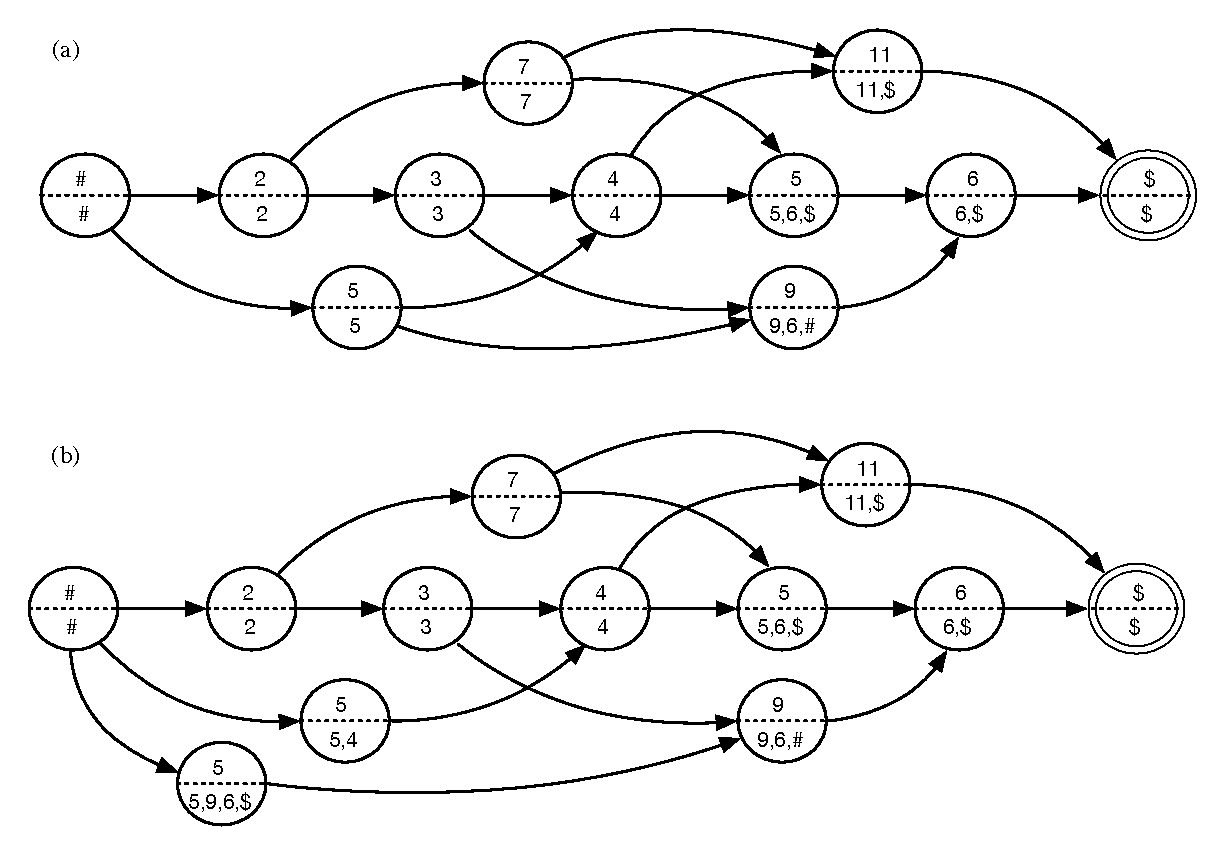
\includegraphics[width=0.6\textwidth]{../content/figures/example_combined}
  \caption{(a) shows an example automaton.  The top half of vertices contains the label, which models a fragment size in Kbp.  The common prefixes of all suffixes spelled from a vertex is written in the bottom half.  Note that there is no ordering of vertices such that all their corresponding suffixes are in lexicographic order;  the leftmost vertex labelled with ``5'' spells suffixes beginning ``5,4,...'' as well as the suffix ``5,9,6,\$'' while the rightmost $5$  spells the suffix ``5,6,\$''. (b) shows the prefix sorted automaton corresponding to the one in (a).  The leftmost vertex $5$ has been duplicated and the outgoing edges of the previous version have been divided between the new replacement instances.  This also divides the suffixes spellable from the prior version.  Now the three $5$ vertices can be ordered based on their common prefixes as [``$5$,$4$,...'',``$5$,$6$,\$'', ``$5$,$9$,$6$, \$'']. }
\label{fig:example}
\end{figure*}

\begin{table*}[h!]
\begin{center}
  \begin{tabular}{ccccccccccccc}
  	\hline
		& \$		& 2		& 3		& 4		& 5,4		& 5,6,\$	& 5,9,6,\$	& 6,\$	& 7	& 9,6,\$	& 11,\$	& \# \\
	\hline
$\BWT$	& 6,11	& \#		& 2		& 3,5		& \#		& 4,7		& \#		& 5,9		& 2	& 3,5		& 4,7		& \$ \\
$\M$		& 1		& 10		& 10		& 10		& 1		& 1		& 1		& 1		&10	& 1		& 1 		& 100 \\
$\F$		& 10		& 1		& 1		& 10		& 1		& 10		& 1		& 10		& 1	& 10		& 10		& 1 \\		
	\hline
	\end{tabular}
      \caption{Table listing the three arrays storing the automaton in memory: $\BWT$, $\M$, and $\F$.}
 \label{bwt-table}
\end{center}
\end{table*}


\subsection{Generalized Compressed Suffix Array.}

%It is an extension of the {\em XBW transform}~\cite{xbw}, which is a compressed  index structure for labeled trees that in itself is a generalization of the FM-index~\cite{dag_method}.  It is an extension of the {\em XBW transform}~\cite{xbw}, which is a compressed  index structure for labeled trees that in itself is a generalization of the FM-index~\cite{dag_method}.  

We index the automaton with the GCSA~\cite{dag_method} for efficient storage and path querying.  The GCSA is a generalization of the FM-index for automata and
%---which as previously mentioned, only supports indexing and querying strings. Nonetheless, there are some parallels between the two data structures and 
we will explain the GCSA by drawing on the definition of the (more widely known) FM-index.  As stated in the background section, the FM-index is based on the deep relationship between the $\SA$ and the $\BWT$ data structures of the input string $\X$. The $\BWT$ of an input string is formed by sorting all characters of the string by the lexicographic order of the suffix immediately following each character.  The main properties the FM-index exploits in order to perform queries efficiently are a) $\BWT[i] = \X[\SA[i]-1]$; and 
%b) the index in the $\SA$ that starts with a given symbol can be found from the $\BWT$ index containing that symbol using small auxiliary data structures. 
b) given that $\SA[i] = j$, and $\C[c]$ gives the position of the first suffix in $\SA$ prefixed with character $c$, then using small auxiliary data structures we can quickly determine $k = \C[\BWT[i]] + \rank(\BWT,\BWT[i],i)$, such that $\SA[k] = j-1$.
The first of these properties is simply the definition of the $\BWT$.  The second is, because the symbols of $\X$ occur in the same order in both the single character prefixes in the suffix array and in the $\BWT$, given a set of sorted suffixes, prepending the same character onto each suffix does not change their order. Thus, if we consider all the suffixes in a range of $\SA$ which are preceded by the same symbol $c$, that subset will appear in the same relative order in (another part of) $\SA$: as a contiguous subinterval of the interval that contains all the suffixes beginning with $c$. Thus by knowing where a symbol's run begins in the $\SA$ and the $\rank$ of an instance of that symbol, we can identify the $\SA$ position beginning with that instance from its position in $\BWT$. A rank data structure over the $\BWT$ thus constitutes a compressed version of the suffix array. 
%The FM-index $\LF()$ function computes the $\SA$ position from the $\BWT$ position using these auxiliary data structures.

%Because those suffixes with the same single character left extension would occur in the same order as those suffixes without the extension, there is a relationship between each suffix and the next longer suffix.  
%Because the BWT is created from sorted suffixes, each position in the BWT can be treated as denoting a particular suffix in a suffix array.  The preceeding character of each suffix is also the one found in the BWT itself for the position in the BWT that denotes that suffix.


%The possition in the equivalent suffix array that represents the $c$ extension can be found using two auxiliary data structures: 1) a $C$ array storing the count of all the lexicographically smaller characters in the text, which can be used to find the beginning of that run of suffixes beginning with that character in the suffix array and 2) an $Occ$ array storing for each position in in the BWT, how many instances of a given character preceed that position.  Since these symbols in the BWT are the prefix characters of the suffixes in the suffix array, they will be in the same order as their sorted -1 suffixes, so their relative position gives an offset into the run of that character prefixes in the suffix array.  $Occ$ is equivalent to the \rank of those characters.  These combination of the start of the run in the SA (given by $C$) and the offset into that run (given by $Occ$) allows mapping from positions in BWT that match a suffix to posstions that denote a $c$ extension.  

%If we allow a suffix array to encode rotations instead of suffixes of a text, the sorted set of rotations can form the Burrows-Wheeler Matrix with the last column being the BWT.  The operation for computing the position of a $c$ extension is called LF() for last-to-first, as it takes the position of a character in the last column of this matrix and computes its position in the first column. 

To generalize the FM-index to automata (from strings), we need to efficiently store the vertices and edges in a manner such that the FM-index properties still hold, allowing the GCSA to support queries efficiently.  An FM-index's compressed suffix array for a string $S$ encodes a relationship between each suffix $S$ and its left extension.  Hence, this suffix array can be generalized to edges in a graph that represent a relationship between vertices.  The compressed suffix array for a string is a special case where the vertices are labeled with the string's symbols in a non-branching path. %Now, we will describe this generalization in more detail by describing how to sort all vertices and edges in an automaton using $\BWT$ and two bit arrays.

\paragraph{Prefix-sorted automata.}
Just as backward search for strings is linked to suffix sorting, backward searching in the BWT of the automaton 
requires us to be able to sort the vertices (and a special set of the paths) of the automaton in a particular 
way. In~\cite{dag_method} this property is called {\em prefix-sortedness}. Let $A = (V,E)$ be a finite automaton, 
let $v_{|V|}$ denote its terminal vertex, and let $v \in V$ be a vertex. We say $v$ is {\em prefix-sorted} by 
prefix $p(v)$ if the labels of all paths from $v$ to $v_{|V|}$ share a common prefix $p(v)$, and no path from any 
other vertex $u \ne v$ to $v_{|V|}$ has $p(v)$ as a prefix of its label. Automaton $A$ is prefix-sorted if all 
vertices are prefix-sorted. See Figure~\ref{fig:example} for an example of a non-prefix sorted automaton and a 
prefix sorted automaton. A non-prefix sorted automaton can be made prefix sorted through a process of duplicating 
vertices and their incoming edges but dividing their outgoing edges between the new instances (see~\cite{dag_method}).

Clearly the prefixes $p(v)$ allow us to sort the vertices of a prefix-sorted automaton into lexicographical 
order. Moreover, if we consider the list of outgoing edges $(u,v)$, sorted by pairs $(p(u),p(v))$, they are
also sorted by the sequences $\ell(u)p(v)$, where $\ell(u)$ denotes the label of vertex $u$. This (dual sortedness)
property allows backward searching to work over the list of vertex labels (sorted by $p(v)$) in the same way
that is does for the symbols of a string ordered by their following suffixes in normal backward search for 
strings.

Each vertex has a set of one or more preceding vertices and therefore, a set of predecessor labels in the 
automaton. These predecessor label sets are concatenated to form the $\BWT$. The sets are concatenated the 
order defined by the above mentioned lexicographic ordering of the vertices. Each element in $\BWT$ then 
denotes an edge in the automaton. Another array of bits, $\F$, marks a `1' for the first element of $\BWT$ 
corresponding to a vertex and a `0' for all subsequent elements in that set. Thus, the predecessor labels, 
and hence the associated edges, for a vertex with rank $r$ are $\BWT[\select(r)..\select(r+1)]$. Another 
array, $\M$, stores the out degree of each vertex and allows the set of vertex ranks associated with a $\BWT$ 
interval to be found using $\rank()$ queries.

%\textit{Vertex Representation}
%In order to index the vertices we first construct an unique string, which we refer to as the \emph{common prefix}, and associate each vertex with respect to that string. This association will allow the vertices to be sorted by their common prefixes and from then on identified by their rank in this sorted order.  To construct the common prefix string, it is important to note that the automaton defines a language comprising a set of strings.  Thus, every path through the automaton corresponds to one of these strings.  If we consider all of the paths that include a particular vertex, we see that the vertex will also be the initial symbol of a suffix for each path.  Those suffixes will have a common prefix--even if it is just the node label itself--which is the common prefix string. 
%
%These common prefixes may not be sufficient to sort vertices as necessary.  In some cases, two vertices may share a property that all paths reachable from one are lexicographically smaller than all paths reachable from the other.  A vertex that shares this property with every other vertex is prefix sorted.  An automaton where every vertex is prefix sorted is a prefix sorted automaton.  A non-prefix sorted automaton can be made prefix sorted through a process of duplicating vertices and their incoming edges but dividing their outgoing edges between the new instances.  See Figure~\ref{fig:example} for an example of a non-prefix sorted automaton and a prefix sorted automaton.  The common prefix of these vertices will then be longer, and with sufficient repetitions of this process, a non-prefix sorted automaton will become prefix sorted. Thus, in order to ensure the vertices can be identified by their rank in sorted order, we construct the automaton so that it is prefix sorted. 
%
%\textit{Edge Representation}
%Each vertex has a set of one or more preceding vertices and therefore, a set of predecessor labels in the automaton.  These predecessor label sets are concatenated to form the $\BWT$ array.  
%The sets are concatenated in an order defined by the above mentioned lexicographic ordering of the vertices.
%%The order of concatenation among these sets is based on the aforementioned lexicographic rank of the successor of each set. 
%Each element of $\BWT$ then denotes an edge in the automaton.  Another array of bits, $\F$, marks a `1' for the first element of $\BWT$ corresponding to a vertex and a `0' for all subsequent elements.  Thus, the predecessor labels, and hence the associated edges, for a vertex with rank $r$ are $\BWT[\select(r)..\select(r+1)]$. Another array, $\M$, stores the out degree of each vertex and allows the set of vertex ranks associated with a $\BWT$ interval to be found using $\rank()$ queries.
%%A bit vector, $F$, is used to encode the mapping from vertex space to edge space, and a bit vector, $M$, is used to map from edge space back to vertex space.  Equivalently, these encode the in-degree and out-degree of the vertices.
%%Since there can be multiple characters preceeding a vertex (and thus all reachable paths from that vertex), a bit vector $F$ encodes with a '1' the first symbol in the BWT array which preceedes a common prefix vertex.  It allows us to map from  multiple BWT positions to a single SA position.  Just as with compressed suffix arrays, the actual suffix array is not stored in memory.% FIXME: describe M bit vector operation
%

% An automaton may be such that the possible suffixes reachable from two or more vertices, when sorted, have overlapping ranges (e.g. A path prefix vertex ``12'' may be followed by either a ``5'' or a ``9'' in one part of the automaton while ``12'' may be followed by either a ``4'' or a ``7'' elsewhere.  These vertices cannot be sorted according to the lexicographic order of reachable paths.)   To induce the required property of a definite ordering, we can modify the automaton by replacing vertices with short common prefixes using new vertices with longer, more specific, common prefixes (e.g. replace the original ``12'' prefix vertex with a ``125'' and a ``129'' vertex, and the latter with ``124'' and ``127'', thus these four vertices can be ordered.).  As vertices denoting short path prefixes are replaced with several longer path prefix vertices, eventually a definite ordering is induced.    This is called {\em prefix doubling}.

%Siren et al.~\cite{dag_method} show that the GCSA can be constructed in $O(|V|+|E|)$ time and space, where $|V|$ is the number of vertices in the automaton and $|E|$ is the number of edges. %Hence, it follows from this result that the automaton for the Rmap data can be constructed in $O(XX)$-time and $O(XX)$-memory.   
 %FIXME: this needs more work

%I don't think you need this --> In this discussion, we assume that the automaton was ensured to be reverse deterministic such that any member of $\Sigma$ only exists once labeling a predecessor vertex of each vertex.

% FIXME: look up proper orthographic form for burrows wheeler



%An FM-index allows exact string search because it encodes the relationship between each pair of consecutive symbols in a text.  The generalization of the GCSA is that the encoded relationship is between vertices in a directed graph.  Under this generalization, an FM-Index is just the special case of a graph formed where every symbol has a single in edge that originates at its predecessor in the text and a single out edge destined for its successor in the text.  The GCSA still includes the BWT component, and like FM-index backward search, an interval on a BWT can denote a subset of the indexed data.  

%In the FM-index, this interval has an equivalent interpretation in a suffix array and in this interpretation, a prefix of all strings in the interval match the suffix of the query searched up to that point.  In the GCSA, each element in the BWT corresponds to vertex in an automaton.  Each vertex has an annotated string indicated the longest common prefix of all strings reachable from it moving forward.  The interval then encodes all vertices whose prefix is consistent with the portion of the query matched up to that point.  

%After the construction of the GCSA, a wavelet tree $\M$ is created that allows us to map from positions in $\R_q$ to positions in $\R^*$ in constant time.

 
%Additional vertices are added to represent hypothetical fragments that could exist for every boundary between two (or more) fragments formed by successful enzyme digestion.  The hypothetical vertices of two combined fragments provide  alternative path segments (consisting of single vertices) around pairs of vertices in the backbone.


\subsection{Exact Matching: GCSA Backward Search.}

%Recall that our aim to find all $\R_i$ in the target database whose alignment to $\R_q$ has a Chi-square statistic less than $\rho_U$, and a ratio of matched to missed restriction sites greater than $\rho_L$.  

Exact matching with the GCSA is similar to the standard FM-index backward search algorithm. As outlined in the background section, FM-index backward search proceeds by finding a succession of lexicographic ranges that progressively match longer and longer suffixes of the query string, starting from the rightmost symbol of the query. The search maintains two items --- a lexicographic range and an index into the query string --- and the property that the path prefix associated with the lexicographic range is equal to the suffix of the query marked by the query index. Initially, the query index is at the rightmost symbol and the range is $[1..n]$ since every path prefix matches the empty suffix.  The search continues using GCSA's backward search step function, which takes as parameters the next symbol (to the left) in the query (i.e. fragment size in $\R_q$) and the current range, and returns a new range.  The query index is advanced leftward after each backward search step.  In theory, since the current range corresponds to a consecutive range in the $\BWT$, the backward search could use use $\select()$ queries on a bit vector $\F$ to determine all the edges adjacent to a given vertex and then two FM-index $\LF()$ queries are applied to the limits of the current range to obtain the new one.  GCSA's implementation uses one succinct bit vector per alphabet symbol to encode which symbols precede a given vertex instead of $\F$.  Finally, this new range, which corresponds to a set of edges, is mapped back to a set of vertices using $\rank()$ on the $\M$ bit vector.


%Each additional symbol in the query string is matched in a process taking two arguments: 1) a lexicographic range, the $\Y$-interval, corresponding to the suffixes in the text, $\ell$, whose prefix matches a suffix of the query string, and 2) an extension symbol $c$.  The process returns a new interval, the $c\Y$-interval, where the prefix of each text suffix corresponding to the new interval is a left extension of the previous query suffix. This works because each prefix of an alignment is also an alignment, including the base case of an empty prefix.





\subsection{Inexact Matching: GCSA Backward Search Using a Wavelet Tree.}


%We emphasize that for ease of exposition, the description of our modifications to and use of the GCSA in the remainder of this section  avoid specific differences between GCSA-based backward search and FM-index backward search. We thus talk about backward searching in the  GCSA as operations on the $\BWT$ of $\R^*$, etc.. We refer the reader interested in the fine-grained differences between the GCSA and FM-index to~\cite{dag_method}. 
% Muggli et al.~\cite{wabi2014} showed that a wavelet tree can efficiently find suitably sized substitute fragments over a large alphabet, but its basic FM-index structure cannot encode alternative compound fragments as substition candidates in light of missing site errors.

% C: this paragraph is too long, make shorter or split in two
%As previously mentioned,  GCSA was developed for sequences on a nucleotide alphabet.  

We modified backward search in the following ways:
(1) we used a wavelet tree to allow efficient retrieval of substitution candidates; (2) we modified the search process to combine consecutive query fragments into compound fragments so as to match fragments in $\R^*$ missing the interposing restriction site; and (3) we introduced backtracking, in order to try substitution candidates and combinations of compound fragment. These modifications are further detailed below.

First, in order to accommodate possible errors in fragment size, we determine a set, $\D$, of candidate fragment sizes that are similar to the next fragment of $\R_q$ to be matched in the query. These candidates are determined by enumerating the distinct symbols in the currently active backward-search range of the $\BWT$ using the wavelet tree algorithm of Gagie et al.~\cite{GNPtcs11}.  This requires introducing bit array $\F$ into the actual implementation\footnote{Recall that this active range, when applied to a lexicographic range, represents the suffixes whose prefixes are the matched portion of the query, while the same range of the $\BWT$ contains possible extension symbols.}. To accommodate possible restriction sites that are present in the query Rmap but absent in target Rmaps, we generate compound fragments (i.e. new symbols) by summing pairs and triples of consecutive query fragment size and then querying the wavelet tree for substitutions of these compound fragments. This summing of multiple consecutive fragments is complementary to the skip vertices in the target automaton and accommodates missed restriction sites in the target, just as the skip vertices accommodate missed sites in the query.  %We remove small fragments with a larger threshold than used for skip edge introduction.  This ensures no need for complementary handling of inconsistent desorption.


%We introduce skip {\emph edges} to provide paths around small target fragments which may be missing in the query.  We filter out small query fragments using a larger threshold to bias toward this scenario. 

%Similarly, small fragments may sometimes be subject to desorption in either the query or the target.
%SJP: found this next part a little wordy:
%One could simply prune all the fragments below a certain threshold size; however, due to the sizing error, one cannot discard based on the true fragment size and one would certainly not achieve consistent discarding across all Rmaps (e.g. a small fragment in two maps covering the same genomic region may be above the threshold in one map and below in another, leading to inconsistent discarding).  Therefore, to find all alignments, 
%and so
%some mechanism to allow inconsistent inclusion of small fragments is required.
%In order to allow inconsistent inclusion between query and target, we introduce skip edges.  These allow paths around small fragments found in the target that might be missing from a query Rmap.  We filter small fragments from the query using a larger threshold, introducing a bias so that skip edges alone suffice for matching.
%Normally, one might need to include skipping over small fragments in not just the target, but in the query as well. This would however result in further branching and slow down the search.  As an alternative, we use separate thresholds for the query and the target so that we can ensure that if a given genomic fragment only is retained in one sequence, it will be retained in the target. 
%FIXME: EXPLAIN WHY.

%SJP: this next paragraph is not super clear.  MDM: It may not be critical; I think there is an interesting insight/way to view this, but it probably should be in discussion. Commenting it out for now.
%% In fact, the search will potentially consider the equivalent of all the paths that exist in the automaton for that same Rmap.  This could be implemented by doing a depth first traversal of $\R_q$'s subgraph in the automaton (locating its backbone and all corresponding skip vertices and edges), however our implementation reconstructs these paths from the query directly. 
%% (This reduces the problem to finding a common path between an automaton for a query and the automaton of the concatenated target Rmaps.) 
%% This traversal only continues as long as there are some paths in the automaton for which the query path comprising the set of compound or original fragments in the query are a statistically plausible match.  Also note that every possible optimal path in a dynamic programming matrix has a corresponding path through the two automata (the actual one indexed by GCSA and the virtual one generated on the fly from $\R_q$).  


 
% As with other FM-index based searches, the target Rmaps are searched in parallel by means of the match interval to the extent they are similar; however, without quantization, the branching factor can be extremely high for the search for substitutions in early fragments from the query.
% SJP: someone left the commment:... [AND SOMETHING LINKING TO PARARLLELIZATION] --- but we don't need to in this context. We're not talking about parallel processing, but rather the multiple alignments that backward search is able to arrive at in a single search process. These are effectively found "in parallel"  
%To reduce the branching factor we quantize the fragment sizes. 
%We thus quantize the data by building a wavelet tree on all Rmaps and then using a wavelet tree traversal.  In particular, we use the algorithm of Gagie et al.~\cite{GNPtcs11}, which takes $O(|D|\log(f/\Delta))$-time to do the wavelet tree quantization, with $|D|$ is the number of candidate match fragment sizes, $f$ is BLAH and FOO is BLAH. IF UNCOMMENTED, ENSURE DELTA USE HERE DOESN'T CLASH WITH OTHER USE IN THE TEXT -mm
%We also use a wavelet tree on the $\BWT$ or $\R^*$ (and the traversal algorithm of Gagie et al.~\cite{GNPtcs11}) in order to explore the neighborhood of candidate matches efficiently, avoiding enumeration of the entire alphabet at each step of the backward search. These candidates are chosen to be within a noise tolerance $t$.  

%[WHAT IS $\R^*$]
%%sjp: it is the concatenation of the Rmaps. It is defined earlier in this section, so this is fine. 
Lastly, since there may be multiple match candidates in the $\BWT$ interval of $\R^*$ 
for a compound fragment drawn from $\R_q$, we add backtracking to backward search so that each candidate size returned to the search algorithm from the wavelet tree is evaluated; i.e., for a given compound fragment size $f$ generated from $\R_q$, every possible candidate fragment size, $f'$, that can be found in $\R^*$ in the range $f - t \ldots f + t$ and in the interval $s \ldots e$ (of the $\BWT$ of $\R^*$) for some tolerance $t$ is used as a substitute in the backward search. Each of these candidates is then checked to ensure that the longer partial alignment formed by a left extension would still satisfy alignment criteria.  This requires the alignment criteria be \emph{monotone}, that is, that the prefixes of a credible long alignment are also credible alignments.  Since the chi-square and binomial CDF statistics are p-values, they make suitable alignment criteria.   When this criteria is still satisfied after including a candidate symbol, it is used as the extension symbol in the backward search.
%This neighborhood is chosen to be within a radius of six standard deviations about the query symbol, since the query and target fragments may be three standard deviations away from the actual fragment size in the genome. 
 
% $\dopp$ additionally combines sequences of fragments in the query to form hypothetical fragments, to allow known fragments in the query to be missing in the target. 
 




%%SJP: moved this subsection to the appendix for RECOMB-seq, see appendix.tex
%\subsection{Practical Considerations}
%
%\textit{Pruning Queries}
%
%One side effect of summing consecutive fragments in both the search algorithm and the target data structure is that several successive search steps with agreeing fragment sizes will also have agreeing sums of those successive fragments.  In this scenario, proceeding deeper in the search space will result in wasted effort. 
%To reduce this risk, we maintain a table of scores obtained when reaching a particular lexicographic range and query cursor pair. We only proceed with the search past this point when either the point has never been reached before, or has only been reached before with inferior scores.
%
%\textit{Wavelet Tree Cutoff}
%The wavelet tree allows efficiently finding the set of vertex labels that are predecessors of the vertices in the current match interval intersected with the set of vertex labels that would be compatible with the next compound fragment to be matched in the query.  However, when the match interval is sufficiently small ($ < 750 $) it is faster to scan the vertices in $\BWT$ directly.
%
%\textit{Quantization}
%The alphabet of fragment sizes can be large considering all the measured fragments from multiple copies of the genome.  This can cause an extremely large branching factor for the initial symbol and first few extensions in the search.  To improve the efficiency of the search, the fragment sizes are initially quantized, thus reducing the size of the effective alphabet and the number of substitution candidates under consideration at each point in the search.  Quantization also increases the number of identical path segments across the indexed graph which allows a greater amount of candidate matches to be evaluated in parallel because they all fall into the same $\BWT$ interval during the search.  This does, however, introduce some quantization error into the fragment sizes, but the bin size is chosen to keep this small in comparison to the sizing error.
%


%\end{methods}


%\section{Discussion}
%\section{Results} \label{sec:results} 

\subsection{Datasets} \label{subsec:data}

Our first dataset consists of approximately 6.9 million paired-end 101 bp reads from the prokaryote genome {\em Francisella tularensis}, generated by Illumina Genome Analayzer (GA) IIx platform. 
It was obtained from the NCBI Short Read Archive (accession number SRR063416). The reference genome was also downloaded from the NCBI website (Reference genome NC\_006570.2).  
The {\em  Francisella tularensis} genome is 1,892,775 bp in length. As a measure of quality assurance, we aligned the reads to the {\em Francisella tularensis} genome using BWA (version 0.5.9) \cite{bwa} with default parameters.  
We call a read {\em mapped} if BWA outputs an alignment for it and {\em unmapped} otherwise.  
Analysis of the alignments revealed that 97\% of the reads mapped to the reference genome, representing an average depth of approximately $367\times$.  

Our second dataset consists of approximately  31.3 million paired-end 100 bp reads from the loblolly pine  ({\em Pinus taeda} L.) genome~\cite{pine}.  
We downloaded the reference genome from the pine genome website~\cite{pinetreeweb} and simulated reads from the largest five hundred scaffolds from the reference using ART~\cite{art} (art illumina). 
% FIXME: What does the read simulator do with runs of N's in scaffolds?  How do these affect our pipelines?
ART was ran with parameters that simulated 100 bp paired end reads with 200 bp insert size and 50x coverage.  
The substitution error rate was reduced to one 10th of the default profile.  
The data for this experiment is available on the $\sequel$ website.  
We simulated an optical map using the reference genome for {\em Francisella tularensis} and loblolly pine since there is no publicly available one for these genomes.  


%Our second dataset consists of approximately 6.9 million paired-end 100 bp reads from the prokaryote genome {\em Porphyromonas gingivalisi}, generated by Illumina Genome Analayzer (GA) IIx platform. It was obtained from the NCBI Short Read Archive (accession number SRR413299). The reference genome was also downloaded from the NCBI website (Reference genome NC\_002950.2).  The {\em  Porphyromonas gingivalisi} genome is 2,343,476 bp in length. As a measure of quality assurance, we aligned the reads to the reference genome using BWA (version 0.5.9) with default parameters~\cite{bwa}.   This analysis of the alignments revealed that 98\% of the reads mapped to the reference genome, representing an average depth of approximately $404\times$.  


\begin{table}[h!]
\begin{center}
\caption{The performance comparison between major assembly tools on the \emph{Francisella tularensis} dataset  (1,892,775 bp, 6,907,220 reads, 101 bp)  using QUAST in default mode \cite{quast}. 
All statistics are based on contigs no shorter than 500 bp. N50 is defined as the length for which the collection of all contigs of that length or longer contains at least half of the sum of the lengths of all contigs, and for which the collection of all contigs of that length or shorter also contains at least half of the sum of the lengths of all contigs.  
\# unaligned is the number of contigs that did not align to the reference genome, or only partially aligned (part).  
Total is sum of the length of all contigs. 
MA is the number of (extensively) misassembled contigs.  
local MA is the total number of contigs that had local misassemblies. 
MA (bp) is the total length of the MA contigs.  
GF is the genome fraction percentage, which is the fraction of genome bases that are covered by the assembly. 
--rr and ++rr denotes before and after repeat resolution, respectively.}
\begin{tabular}{|c|c|c|c|c|c|c|c|c|c}
\hline
\textbf{Assembler} 			&{\bf \# contigs }		& \textbf{N50}	& \textbf{Largest (bp)}	& \textbf{Total (bp) }	&\textbf{MA}	&\textbf{local MA}	& {\bf MA (bp)} 		& \textbf{GF (\%)} \\ 
 						&{\bf (\# unaligned) }		& 			& 					& 				&			& 			& 				& \\ \hline
Velvet					& 358 (3 + 35 part)		& 7,377		& 39,381				& 1,762,202 		& 11			& 36			& 84,965			& 92.09			  \\ \hline
SOAPdenovo 				& 307 (3 + 31 part)		& 8,767		& 39,989				& 2,018,158 		& 10			& 35			& 96,258			& 92.05				\\ \hline
ABySS					& 96 (1 part)  			& 27,975  		& 88,275				& 1,875,628		& 64  		& 32			& 1,330,684		& 95.87  			 	 \\ \hline
SPAdes (--rr)				& 102 (2 + 11 part) 		&  25,148		& 87,449				& 1,788,634		& 11 			& 30			& 258,309			& 92.81			 	 \\ \hline
SPAdes (+rr)				& 100 (2 + 17 part) 		&  26,876		& 87,891				& 1,797,197 		& 23 			& 31			& 497,356			& 93.75			 	 \\ \hline
IDBA						& 109 (1 + 10 part)		& 23,223 		& 87,437 				& 1,768,958		& 10			& 31			& 221,087			& 92.64  				 \\ \hline
%HyDA					& 					&			&  					&  				&  			&			&				& 			 	 \\ \hline
\end{tabular}
\label{tab:ging}
%\end{center}
%\end{table}
%\begin{table}[ht!]
%\begin{center}
\vspace{10mm}
\caption{\footnotesize{The performance comparison between major assembly tools on Loblolly pine ({\em Pinus taeda} L.) genome dataset (62,647,324 bp, 31.3 million reads, 100 bp) using QUAST in default mode \cite{quast}.}}
\label{tab:pine}
\begin{tabular}{|c|c|c|c|c|c|c|c|c|c}
\hline
\textbf{Assembler} 			&{\bf \# contigs }		& \textbf{N50}	& \textbf{Largest (bp)}	& \textbf{Total (bp) }	&\textbf{MA}	&\textbf{local MA}	& {\bf MA (bp)} 		& \textbf{GF (\%)} \\ 
 						&{\bf (\# unaligned) }		& 			& 					& 				&			& 			& 				& \\ \hline
Velvet					& 13,327 (0)			& 1,740		& 10,823				& 51,851,131 		& 0			& 0			& 0				& 62.21			  \\ \hline
SOAPdenovo 				& 16,126 (0 + 1 part)		& 7,950		& 63,004				& 57,205,817 		& 0			& 0			& 0				& 90.01				\\ \hline
ABySS					& 4,586 (16 + 89 part)  	& 37,089  		& 201,382				& 63,349,408		& 127  		& 715		& 1,391,565		& 98.17  			 	 \\ \hline
SPAdes (--rr)				& 20,671 (4 + 10 part) 	& 4,809		& 44,993				& 45,079,764		& 7 			& 11			& 65,079			& 81.30			 	 \\ \hline
SPAdes (+rr)				& 8,607 (7 + 102 part) 	& 16,957		& 108,442				& 59,730,939 		& 299 		& 57			& 3,734,609		& 94.57			 	 \\ \hline
IDBA						& 22,409 (3 + 31 part)	& 3,990 		& 40,213				& 49,765,854		& 61			& 200		& 292,769			& 79.03  				 \\ \hline
\end{tabular}
\end{center}
\end{table}


We assembled both sets of reads with a wide variety of state-of-the-art assemblers.  The versions used were those that were publicly available before or on September 1, 2014: 
%These were: 
SPAdes (version 3.1)~\cite{spades}; Velvet (version  1.2.10)~\cite{Zerbino:2008}; SOAPdenovo (version 2.04)~\cite{soap}; ABySS (version 1.5.2)~\cite{Simpson:2009}; and IDBA-UD (version 1.1.1)~\cite{idbaud}.
SPAdes outputs two assemblies: before repeat resolution and after repeat resolution --- we report both.
Some of the assemblers emitted both contigs and scaffolds.  We considered contigs only but note that all scaffolds had a greater number of misassembly errors. 
{\em We emphasize that our purpose here is not to compare the various assemblers, but demonstrate that all assemblers produce misassembly errors, which are in need of consideration and correction.  } 

We used Quast \cite{quast} in default mode to evaluate the assemblies.  
Quast defines misassembly error as being {\em extensive} or {\em local}.  
A (extensive) misassembled contig is defined as one that satisfies one following conditions:  (a) the left flanking sequence aligns over 1 kbp away from the right flanking sequence on the reference; (b) flanking sequences overlap on more than 1 kbp; (c) flanking sequences align to different strands or different chromosomes. 
Whereas, a local misassembled contig is one that satisfies the following conditions: (a) two or more distinct alignments cover the breakpoint; (b) the gap between left and right flanking sequences is less than 1 kbp; and the left and right flanking sequences both are on the same strand of the same chromosome of the reference genome.  
We made a minor alteration to Quast to output which contigs contain local misassembly errors.  
A contig can contain both extensive and local misassembly errors.  
Any correctly assembled contig is one that does not contain either type of error.  

\subsection{Detection of Misassembly Errors in {\em Francisella tularensis}} \label{sec:tularensis}

Table~\ref{tab:ging} gives the assembly statistics corresponding to this experiment.  
Comparable assembly results on this data were reported by Ilie et al.~\cite{sage}, though in some cases we used more recent software releases (e.g., for SPAdes).  
Note that the number of locally misassembled contigs and the number of extensively misassembled contigs is not disjoint.
A contig can be locally and extensively misassembled.   
Thus, Table \ref{tab:ging} gives the number of contigs having at least one extensive misassembly error, and the number of contigs having at least one local misassembly error.

\begin{table}[h!]
\begin{center}
\caption{The performance comparison of our method on the \emph{Francisella tularensis} dataset. 
The true positive rate (TPR) in this context is a contig that is misassembled and is predicted to be so. 
The false positive rate (FPR) is a correctly assembled contig that was predicted to be misassembled.
The TPR and FPR is given as a percentage with the raw values given in brackets}
{\setlength{\tabcolsep}{1em}
\begin{tabular}{|l|c|c|c|c|}
\hline
\textbf{Correction Method}								& \textbf{Assembler}		&{\bf MA TPR}			& {\bf local MA TPR}		& \textbf{FPR}	\\ \hline
							& Velvet				& 100\% (11 / 11)		& 100\% (36 / 36)		& 58\% (180 / 312)		\\ 
							& SOAPdenovo		& 100\% (10 / 10)		& 100\% (35 / 35)		& 63\% (165 / 263)	\\ 
 misSEQuel								& ABySS				& 100\% (64 / 64)		& 100\% (32 / 32)		& 87\% (20 / 23)			\\ 
(paired-end data only)				& SPAdes (--rr)			& 100\% (11 / 11)		& 100\% (30 / 30)		& 83\% (52 / 63)		\\ 
							& SPAdes (++rr)		& 100\% (23 / 23)		& 100\% (31 / 31)		& 86\% (49 / 57)		\\ 
							& IDBA				& 100\% (10 / 10)		& 100\% (31 / 31)		& 38\% (57 / 149) \\ \hline \hline
				
							& Velvet				& 55\% (6 / 11)			& 69\% (25 / 36)			& 24\% (76 / 312)	\\ 
							& SOAPdenovo		& 80\% (8 / 10)			& 63\% (22 / 35)			& 29\% (77 / 263)	\\ 
misSEQuel					& ABySS				& 69\% (44 / 64)		& 88\% (28 / 32)			& 13\% (3 / 23)		\\ 
(optical mapping data only)		& SPAdes (--rr)			& 91\% (10 / 11)		& 87\% (26 / 30)			& 21\% (13 / 63)		\\ 
							& SPAdes (++rr)		& 87\% (20 / 23)		& 81\% (25 / 31)			& 16\% (9 / 57)			\\ 
							& IDBA				& 90\% (9 / 10)			& 77\% (24 / 31)			& 10\% (15 / 149)		\\ 
\hline \hline
					
							& {\bf Velvet}					& {\bf 55\% (6 / 11)}			& {\bf 100\% (26 / 36)}		&	{\bf 22\% (68 / 312)}	\\ 
							& {\bf  SOAPdenovo}				& {\bf 80\% (8 / 10)}			&{\bf 84\% (21 / 35)}			&	{\bf 20\% (53 / 263)}	\\
 {\sc\bf misSEQuel}				& {\bf ABySS}					& {\bf 69\% (44 / 64)}			& {\bf 88\% (28 / 32)}			&	{\bf 13\% (3 / 23)}		\\ 
{\bf (paired-end and optical}	& {\bf  SPAdes (--rr)}				&{\bf 91\% (10 / 11)}			& {\bf 87\% (26 / 30)}			&	{\bf 19\% (12 / 63)}		\\ 
{\bf mapping data)}				& {\bf SPAdes (++rr)}				&{\bf 97\% (20 / 23)}			& {\bf 81\% (25 / 31)}			&	{\bf 16\% (9 / 57)}		\\ 
							& {\bf IDBA}					&{\bf 90\% (9 / 10)}			&{\bf  77\% (24 / 31)}			&	{\bf 9\% (14 / 149)}		\\ 
\hline \hline
							& Velvet						& 55\% (6 / 11)		& 11\% (4 / 36)				& $<$ 1\% (2 / 312)		\\ 
							& SOAPdenovo				& 20\% (2 / 10)		& 14\% (5 / 35)				& 2\% (6 / 263)	\\  
REAPR						& ABySS						& 13\% (8 / 64)		& 13\% (4 / 32)				& 4\% (1 / 23)			\\  
							& SPAdes (--rr)					& 27\% (3 / 11)		& 27\% (8 / 30)				& 5\% (3 / 63)			\\ 
							& SPAdes (++rr)				& 0\% (0 / 23)		& 19\% (6 / 31)				& 11\% (6 / 57)		\\
							& IDBA						& 40\% (4 / 10)		& 13\% (4 / 31)				& 4\% (6 / 149)			\\ 
\hline
\end{tabular}}
\label{tab:roc}
\end{center}
\end{table}



Table \ref{tab:roc} shows the results for: (a) $\sequel$ with paired-end data only; (b) $\sequel$ with optical mapping data only; and (c) $\sequel$ with both optical mapping and paired-end data in order to demonstrate the gain of combining both types of data.  
As demonstrated by these results, using short read paired-end data alone produces a high false positive rate, since it is unable to distinguish between structural variations within the genome and misassembly errors.  
This is an inherent shortcoming of short read data and demonstrates that in order to decrease the false positive rate, another source of information must be used in combination.
Optical mapping data has a much lower false positive rate and when used in combination with paired-end data, produces optimal results.  The lowest false positive rate was witnessed when both optical mapping and paired-end data were used.  In some cases, the reduction in the false positive rate was dramatic; from 87\% (ABySS, paired-end data) to 13\% (ABySS, paired-end and optical mapping data).  The true positive rate of locally misassembled contigs was between 77\% and 100\% when both paired-end and optical mapping data were used.  Lastly, true positive rate of extensively misassembled contigs was between 55\% and 100\% when both paired-end and optical mapping data were used. 

In our experiments, we iterate through combinations of three enzymes from the REBASE enzyme database \cite{roberts2010rebase} and use the set of enzymes that performed best.  
Our results demonstrate that with a good enzyme choice over half of all extensively misassembled contigs, and over 75\% of locally misassembled contigs can be identified with only a 9\%-22\% false discovery rate.
 
\subsection{Detection of Misassembly Errors in Loblolly Pine}\label{sec:pine}

The results for the loblolly pine are shown in Table \ref{tab:roc_pine}.  Both Velvet and SOAPdenovo produced zero misassembled contigs on this dataset, so we do not include them in Table~\ref{tab:roc_pine}.
% just shows results for the remaining assemblies.
$\sequel$ correctly identifies between 31\% and 100\% of extensively misassembled contigs, and between 57\% and 73\% of locally misassembled contigs.  The false positive rate was between 0.6\% and 43\%.  Although, REAPR has a lower false positive rate (between 3\% and 11\%), it is only capable of identifying a small number of extensively misassembled contigs (between 2\% and 14\%) and a small number of locally misassembled contigs (between 2\% and 27\%).  

Lastly, the restriction enzymes used in our experiments were chosen to be optimal by considering the set of all possible enzymes in the aformentioned database.  
Nonetheless, we note that if the enzyme combination was chosen at random then the expected false positive rate and true positive rate would decrease by a small fraction for majority of the assemblies considered.  
See the Appendix for prototypical ROC curves and heatmaps illustrating the density of enzyme combinations at various detection rates.



\begin{table}[h!]
\begin{center}
\caption{The performance comparison of our method on the loblolly pine dataset. 
Again, a true positive in this context is a contig that is misassembled and is predicted to be so. 
A false positive is a correctly assembled contig that was predicted to be misassembled.}
{\setlength{\tabcolsep}{1em}
\begin{tabular}{|l|c|c|c|c|}
\hline
\textbf{Correction Method}& \textbf{Assembler} 		&{\bf MA TPR}				& {\bf local MA TPR}					& \textbf{FPR}	 \\ \hline
 					& {\bf ABySS}				&  {\bf 31\% (40 / 127)}		&  {\bf 57\% (405 / 715)} 		  	 	& {\bf 43\% (1,604 / 3,754)}		 	 \\ 
{\sc\bf misSEQuel}		& {\bf SPAdes (--rr)}			&  {\bf 100\% (7 / 7)}			&  {\bf 73\% (8 / 11)}			 		& {\bf $<$1\% (135 / 20,653)	}	 	 \\ 
					& {\bf SPAdes (+rr)}			&  {\bf 67\% (199 / 299)}		& {\bf 67\% (38 / 57)}			 		& {\bf 38\% (3,117 / 8,254)} 		 	 \\ 
					& {\bf IDBA}				&  {\bf 52\% (32 / 61)}		&  {\bf 73\% (145 / 200)} 		  	 	& {\bf 19\% (4,258 / 22,150)}			 \\ 
\hline 
					& ABySS					& 7\% (9 / 127) 				& 2\% (12 / 715) 		  			& 3\% (112 / 3,754)		 \\  
 REAPR				& SPAdes (--rr)				& 14\% (1 / 7)				& 27\% (3 / 11)		 				& 6\% (1,323 / 20,653)		 	 \\ 
					& SPAdes (+rr)				& 7\% (21 / 299)			& 5\% (3 / 57)		 				& 5\% (424 / 8,254)	 \\ 
					& IDBA					& 2\% (1 / 61)				& 6\% (12 / 200)		  	 		&11\% (2,354 / 22,150)		 \\  
\hline
\end{tabular}}
\label{tab:roc_pine}
\end{center}
\end{table}


\subsection{Practical Considerations: Memory and Time} \label{mem_time}

We evaluated the memory and time requirements of $\sequel$.   Since $\sequel$ is a multi-threaded application, its wall-clock-time depends on the computing resources available to the user.  
$\sequel$ required a maximum of 8 threads, 16 GB and 1.5 hours on all assemblies of {\em  Francisella tularensis}, and a maximum of 20 GB and 2.5 hours to complete on all assemblies of loblolly pine.
Most genome assemblers require an incomparably greater amount of time and memory and thus, from a practical perspective, the requirements of $\sequel$ are not a significant increase.  
The difference in the resource requirements of $\sequel$ in comparison to modern assemblers is due to the fact it operates contig-wise rather than genome-wise and therefore, only deals with a significantly smaller portion of the data at a single time.
We conclude by mentioning that $\sequel$ is not optimized for memory and time and both could be further reduced but reimplementing the red-black positional de Bruijn graph using memory and time succinct data structures. 





%\section{Conclusion}
%%\section{Discussion and Conclusions}
\label{sec-discussion}

We demonstrate that $\dopp$ is capable of finding the alignment between any pair of  Rmaps in the June plum data set in less than 67 CPU hours whereas the dynamic programming method of Valouev et al.~\cite{Valouev06} requires 1001 hours of CPU time. This latter method computes the optimal alignment between all prefixes of every pair of Rmaps, while our method succeeds in avoiding this exhaustive computation by using an index data structure to narrow the search to consider a smaller set of plausible alignments only. Hence, although, the dynamic programming methods achieve practical running time on small genomes, they are unlikely to scale to large genomes.   As previously mentioned, the first step in building a genome wide consensus map from the Rmap data is to compute the pairwise alignment among Rmaps, and this is the primary motivation for the development of $\dopp$. This pairwise alignment step is the main computational bottleneck in the consensus map building tool of Valouev et al., and $\dopp$ could easily be substituted for their dynamic programming alignment method, to efficiently compute the consensus map for large genomes, such as plum. 

%In fact, the main goal of the work of Valouev et al. is to build a consensus optical map and its first step---which is the bottleneck in achieving this goal---is to compute the alignment between any pair of Rmaps.  Hence, $\dopp$ could easily be substituted for their dynamic programming alignment method, which would result in an efficient means to compute the consensus map for large genomes, such as plum.  

Taking a broader view, $\dopp$ is simply an error-tolerant index-based alignment program that could have additional purposes beyond Rmap data.  For example, one interesting application of this work would be to align {\em in silico} digested long (PacBio) reads to a genome wide optical map, or to the Rmaps.  This complements the work of  Pendleton et al. \cite{ali}, which scaffolds PacBio data using BioNano Irys data.  Our alignment method could be used to assemble or preprocess PacBio reads that have large errors and should undergo error correction, or to isolate regions in the reads that should undergo error correction.  
%SJP: taking this last part out, I think we make out point already, earlier in the paragraph, and don't need to quote statistics of PacBio, which everyone knows anyway. %The PacBio RS technology generates extremely long reads ($\geq$1,000 bp), but with high single-pass error rates (15\% error rate), and correction of these reads is widely regarded as computationally expensive.  This proposed filtering step could make the error correction process more efficient.  

%We conclude by stating that, in addition to this specific use of $\dopp$ there are many other applications yet to be defined and explored.

%The method presented here occupies a middle ground where missing sites in the target are accomodated by combining fragments in the query and missing sites in the query are accomodated by combining vertex labels in the target automaton. Techniques that accomodate both sets of missing sites in only the query processing or encoded only in the target database may prove fruitful. 

%Our work illustrates the successful adaptation of modern data structures to Rmap alignment, but there is room for innovation in practice.  Sorting query Rmaps would allow the dominant work (exploring prefix matches which do not extend to full query matches) to be shared among all Rmaps sharing common prefixes.  Secondly, a wavelet tree is traversed both to find a candidate set of substitutions and can also be used for rank/select dictionary queries for the backwards search step. It may be fruitful to design an algorithm that shares rank/select work, making a single pass for both these purposes.  Third, indexing Rmaps bidirectionally and searching both ends results in alignments being found twice.  After using an Rmap as a query, it need not exist in the database, and addressing this would halve the total computational work by reporting alignments only once.
 
%Lastly, optical mapping is a relatively new technology, and thus, with so few algorithms available for working with this data, we feel there remains good opportunities for developing more efficient and flexible methods. Dynamic programming optical map alignment approaches are still important today, as the assembly of the consensus optical maps from the individually imaged molecules often has to deal with missing or spurious restriction sites in the single molecule maps when enzymes fail to digest a recognition sequence or the molecule breaks.  Though coverage is high (e.g. about 1,241 Gb of optical data was collected for the 2.66 Gb goat genome), there may be cases where missing restriction site errors are not resolved by the assembly process.   In these rare cases (only 1\% of alignments reported by SOMA on parrot contain such errors) they will inhibit $\twin$'s ability to find correct alignments.  In essence, $\twin$ is trading a small degree of sensitivity for a huge speed increase, just as other index based aligners have done for sequence data.  Sir\'{e}n et al.~\cite{dag_method} recently extended the Burrows-Wheeler transform (BWT) from strings to acyclic directed labeled graphs and to support path queries. In future work, an adaptation of this method for optical map alignment may allow for the efficient handling of missing or spurious restriction sites.

%I'm not sure if it's punchy, but if all you want to do is know how many approximate matches exist, we can skip the step of converting BWT intervals to original "text" intervals.  There is also the fact that we match all approximate patterns concurrently.  This is the same argument as in BWA which says "Because exact repeats are collapsed on one path on the prefix trie, we do not need to align reads against each copy of the repeat."  In our case, it's not just DNA sequence repeats, but since ORM data has less resolution, there may be multiple non repeat DNA strings that happen to have the restriction enzyme target motif in the same place.
\



%\section*{Acknowledgement}
%The authors would like to thank Journi Sir\'{e}n from the Wellcome Trust Sanger Institute for many insightful discussions concerning the GCSA code base.   
%\paragraph{Funding\textcolon} MM and CB were funded by the Colorado Clinical and Translational Sciences Institute which is funded by National Institutes of Health (NIH-NCATS, UL1TR001082, TL1TR001081, KL2TR001080).  SJP was supported by the Helsinki Institute of Information Technology (HIIT) and by Academy of Finland through grants 294143 and 250345 (CoECGR).  All authors greatly appreciate the funding provided for this project.  


%\bibliographystyle{natbib}
%\bibliographystyle{achemnat}
%\bibliographystyle{plainnat}
%\bibliographystyle{abbrv}
%\bibliographystyle{bioinformatics}
%
%\bibliographystyle{plain}
%
%\bibliography{Document}


\bibliographystyle{plain}
\bibliography{../cdbg}

%% \begin{thebibliography}{}
%% \bibitem[Bofelli {\it et~al}., 2000]{Boffelli03} Bofelli,F., Name2, Name3 (2003) Article title, {\it Journal Name}, {\bf 199}, 133-154.

%% \bibitem[Bag {\it et~al}., 2001]{Bag01} Bag,M., Name2, Name3 (2001) Article title, {\it Journal Name}, {\bf 99}, 33-54.

%% \bibitem[Yoo \textit{et~al}., 2003]{Yoo03}
%% Yoo,M.S. \textit{et~al}. (2003) Oxidative stress regulated genes
%% in nigral dopaminergic neurnol cell: correlation with the known
%% pathology in Parkinson's disease. \textit{Brain Res. Mol. Brain
%% Res.}, \textbf{110}(Suppl. 1), 76--84.

%% \bibitem[Lehmann, 1986]{Leh86}
%% Lehmann,E.L. (1986) Chapter title. \textit{Book Title}. Vol.~1, 2nd edn. Springer-Verlag, New York.

%% \bibitem[Crenshaw and Jones, 2003]{Cre03}
%% Crenshaw, B.,III, and Jones, W.B.,Jr (2003) The future of clinical
%% cancer management: one tumor, one chip. \textit{Bioinformatics},
%% doi:10.1093/bioinformatics/btn000.

%% \bibitem[Auhtor \textit{et~al}. (2000)]{Aut00}
%% Auhtor,A.B. \textit{et~al}. (2000) Chapter title. In Smith, A.C.
%% (ed.), \textit{Book Title}, 2nd edn. Publisher, Location, Vol. 1, pp.
%% ???--???.

%% \bibitem[Bardet, 1920]{Bar20}
%% Bardet, G. (1920) Sur un syndrome d'obesite infantile avec
%% polydactylie et retinite pigmentaire (contribution a l'etude des
%% formes cliniques de l'obesite hypophysaire). PhD Thesis, name of
%% institution, Paris, France.

%% \end{thebibliography}
\end{document}
